%%% -*-LaTeX-*-

\chapter{Theoretical Background on Morse Theory}
\label{ch:theory}

Though we have introduced numerous topological constructs in previous chapters, we now provide a more formal treatment of them in this chapter and discuss implementation issues regarding how to approximate on unstructured datasets existing in the high-dimensional setting.

As we are interested in functional relationships we limit ourselves to Morse theory.
%
Morse theory~\cite{Matsumoto2002,Milnor1973,Morse1949} is a sub-topic of differentiable topology that analyzes the topology of manifolds under differentiable functions.
%
Specifically, a class of functions, so-called Morse functions, are used to study such things as the critical points, level-sets and gradient behavior of manifold spaces.
%
As such, the remainder of this section will address each one of these categories in turn.

\begin{defn}
  \textbf{Morse function} - a smooth function with no degenerate critical points, and every critical point is isolated.
\end{defn}

\section{Critical Points}

\begin{lem} Morse Lemma - Let $\mathbf{p}$ be a non-degenerate critical point of $f : A \rightarrow \mathbb{R}$ where $A$ is an $n$-manifold, then there exists a local coordinate system $(x_1,...,x_n$) in a neighborhood of $\mathbf{p}$ such that $x_i(\mathbf{p}) = 0$ and is represented in a \textbf{standard form}:

\begin{equation}
f = f(\mathbf{p}) - \sum_{i=1}^{\lambda}x_i^2 + \sum_{j=\lambda+1}^n x_j^2, \{\lambda \in \mathbb{Z} | 0 \leq \lambda < n\}
\end{equation}
\end{lem}

This lemma claims that locally around each non-degenerate critical point, we can fit a parabolic function with respect to each dimension to represent $f$ where a given number of dimensions will have downward-facing parabolas and the remaining will have upward-facing parabolas.
%
The parameter $\lambda$ specifies how many of each occur for the given critical point.

\begin{defn}
\textbf{Critical point index} - Given the standard form above for a critical point $\mathbf{p}$, the value of $\lambda$ represents the index of $\mathbf{p}$ for $f$.
\end{defn}

A 0-index critical point represents a local minimum, since locally the function is increasing in every direction about the point. Critical points of index $k$ where $0 < k < d$ and $d$ is the dimension of the manifold are known as $k$-saddles.
%
Saddles are so named for the shape they resemble in the 2-manifold case, and in that case exhibit alternating sign of the directional derivative when traversing a clockwise/counterclockwise path around the saddle.
%
The $d$-index critical points represent local maxima where locally the function is decreasing in every direction. Locally, consider a parabola that opens downward when considering each dimension in isolation.

\begin{figure}[!ht]
  \centering
  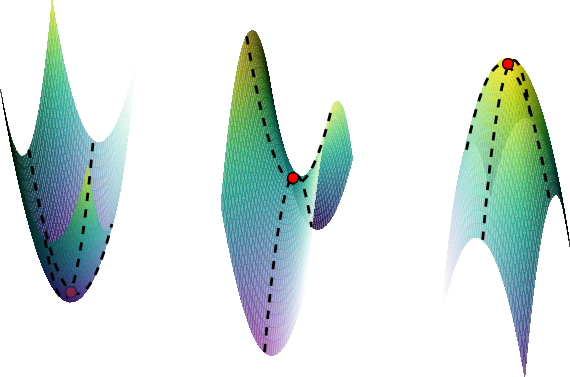
\includegraphics[width=0.5\textwidth]{figs/chap4/criticalPoints}
  \caption[Critical Points of Varying Index]{The standard form of critical points is summarized in the 2D case by visualizing parabolic curves along each dimensional axis. Here we see from left, a 0-index minimum with 0 downward facing parabolas, a 1-saddle with 1 downward facing parabola, and a 2-index maximum with 2 downward facing parabolas.}
  \label{fig:topo-structure}
\end{figure}

\section{Morse and Morse-Smale Complexes}

As stated previously, we can also use Morse theory to partition a space according to uniform gradient flow.
%
For a given location in the domain space, one can follow the gradient direction to a local maximum.
%
Likewise, following the negative gradient direction leads to a local minimum.
%
The path defined by following the gradient in both directions is known as an integral line:

\begin{defn}
  \textbf{Integral line} - A curve, $l(t)$ such that $\frac{d l}{d t}(t) = \nabla f(l(t)), \forall t \in \mathbb{R}$. In words, $l$ is a path whose tangent is parallel to the gradient of $f$ everywhere it is defined.
\end{defn}

\begin{defn}
  \textbf{Origin} - $lim_{t\rightarrow -\infty}l(t)$
\end{defn}

\begin{defn}
  \textbf{Destination} - $lim_{t\rightarrow \infty}l(t)$
\end{defn}

Integral lines on Morse functions have several useful properties:

\begin{itemize}
\item Integral lines are disjoint or the same
\item Integral lines cover all of $\mathbb{M}$
\item Origin and destination of an integral line are critical point of $f$.
\item Integral lines are monotonic and thus $org(l) \neq dest(l)$.
\item Each point in $\mathbb{M}$ has one and only one integral line passing through it.
\end{itemize}

Using the origin or destination as classifiers, we can partition the data into either ascending or descending manifolds which are defined below.

\begin{defn}
  \textbf{Ascending/unstable Manifold} - The set of points in a manifold whose integral lines have the same origin.
\end{defn}

\begin{defn}
  \textbf{Descending/stable Manifold} - The set of points in a manifold whose integral lines have the same destination.
\end{defn}

% \subsection{Morse Complex}

\begin{defn}
 \textbf{Morse Complex} - a partition of a manifold into equivalence classes based on the destination of integral lines: $\{x,y \in A | x~y \Rightarrow dest(x) = dest(y)\}$. Also, the complex of descending manifolds of $f$.
\end{defn}

By inverting the function, $-f$, and computing the Morse complex, we can obtain the complex of ascending manifolds of the original function, $f$.
%
By combining both of these complexes, we can obtain the Morse-Smale complex that partitions the space into areas of distinct origin and destination pairs.

% \subsection{Morse-Smale Complex}

\begin{defn}
\textbf{transverse intersection} - Consider two submanifolds of $\mathbb{C}$, $\mathbb{A}$ and $\mathbb{B}$. $\{\forall \mathbf{x} \in \mathbb{A} \cap \mathbb{B}: T_{\mathbb{A}} + T_{\mathbb{B}} = T_{\mathbb{C}} \text{ or } \mathbb{A} \cap \mathbb{B} = \emptyset\}$ where $T_{X}$ represents the tangent space of $X$.
%
Thus, if $\mathbb{A}$ and $\mathbb{B}$ intersect, they do so such that their combined tangent maps spans the tangent space of the ambient manifold $\mathbb{C}$.
\end{defn}

\begin{defn}
\textbf{Morse-Smale function} - A Morse function whose ascending and descending manifolds interesect transversally.
\end{defn}

\begin{defn}
\textbf{Morse-Smale Complex} - The complex formed by the intersection of the Morse complexes of $f$ and $-f$.
\end{defn}

In this way, a Morse-Smale complex identfies each location in the manifold with a local minimum (origin) and a local maximum (destination).
%
Boundaries between cells in a $d$-manifold are themselves $(d-1)$-manifolds that connect local minima to 1-saddles, 1-saddles to 2-saddles, etc., and $(d-1)$-saddles to local maxima.

% \subsection{Piecewise Linear}

This theory works well when applied to smooth fields, but some gaps must be addressed in order to perform such a decomposition on arbitrary dimensional point cloud data.
%
Namely, in order to identify each point to an ascending or descending manifold, we must trace the integral lines through the available data which implies that we have some connectivity structure among the data points.
%
In order to do this, we employ concepts from discrete Morse theory~\cite{Forman2002}.
%
Gyulassy has addressed many of these issues when working with structured and unstructured grids in low dimensional spaces~\cite{Gyulassy2008}, and more recently Gerber et al.~\cite{GerberBremerPascucci2010} have developed an algorithm for approximating gradient on aribtrary dimensional point clouds.
%
In this work, we utilize the latter algorithm and so explain it in further detail with proposed improvements.

\section{Arbitrary Dimensional Approximation of the Morse-Smale Complex}
\label{sec:approximationMSC}

We treat the problem of computing the Morse-Smale complex as computing two Morse complexes, one to compute descending manifolds (Morse complex of $f$) and another to compute ascending manifolds (Morse complex of $-f$).
%
As mentioned, we must impose a connectivity structure on the data in order to estimate gradient.
%
For this, a neighborhood graph is used which represents a 1-skeleton of the manifold.
%
The original works of Gerber et al.~\cite{GerberBremerPascucci2010,GerberPotter2012,GerberRubelBremer2011} used a $k$-nearest neighbor graph, but we have explored the use of the empty region graphs proposed by Correa and Lindstrom~\cite{CorreaLindstrom2011} which were shown to provide better results in extracting topological features from sparsely sampled data sets.
%
Under specific sampling densities, the $k$-nearest neighbor can tend to bias certain directions where the point density is higher.
%
The empty region graphs, on the other hand, validate edges by ensuring no points lie in a region encompassing the edge.
%
The shape of this region varies according to the specific type of graph used, but the end result is a less biased and more uniform distribution of edges over the hypersphere of directions emanating from any given point.
%
A detailed investigation corroborated these findings and is included in
Section~\ref{paper:TopoInVis2013}.
%
In all of the experiments where this method is employed in this document, we denote the type of graph used.

The algorithm is quite straightforward once the graph is imposed on the data.
%
We visit each point and estimate its positive and negative gradient directions according to the function value difference between itself and each of its neighbors divided by the distance between the two points.
%
The largest magnitude postive and negative values belong to the edges that represent the discretized integral line.
%
If a point has no values of lesser value, it is a local minimum.
%
Equally, if a point has no values of higher value, it is labeled a local maxima.
%
We can then trace the positive integral line from each data point up to a local maximum, and trace the negative integral line down to a local minimum.
%
We retain the indices of the identified local minimum and maximum and this pair of indices represents the Morse-Smale cell to which this point belongs.

Note, that gradient inconsistencies such as crossing integral lines can form if the graph has crossing edges.
%
This can be avoided by detecting and pruning such edges from the graph.
%
In pratical settings, we begin with an approximate $k$-nearest neighbor graph where $k$ is intentionally set higher than expected and prune it with one of the empty region criteria from Correa and Lindstrom's work to achieve computational efficiency.

Figure~\ref{fig:mscAlgorithm} shows the three step process of the discretized Morse-Smale complex algorithm including application of a graph structure, tracing gradients to local extrema, and the third step discussed in the next section, persistence simplification, which essentially denoises the results.

\begin{figure}[!ht]
  \centering
  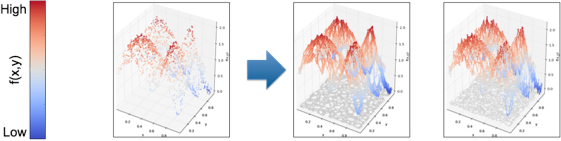
\includegraphics[width=0.65\textwidth]{figs/chap4/amscStep1}
  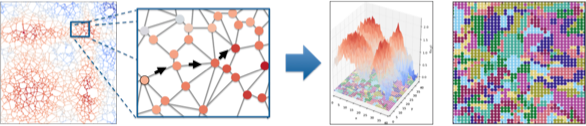
\includegraphics[width=0.65\textwidth]{figs/chap4/amscStep2}
  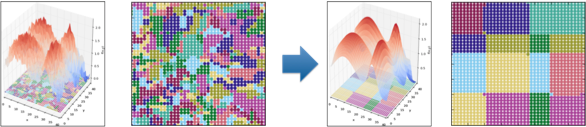
\includegraphics[width=0.65\textwidth]{figs/chap4/amscStep3}
  \caption[Illustration of the Morse-Smale Approximation algorithm for unstructured data]{There are three main steps in the approximation algorithm for computing the Morse-Smale complex. They are from top to bottom: construction of graph on input data, gradient tracing to local extrema, and construction of hierarchy of features allowing for simplification of the extracted topology.}
  \label{fig:mscAlgorithm}
\end{figure}

\section{Persistence Simplification}


%%TODO: I think this last part will include the contour tree, so I should mention how it is used in high-dimension, right?
% \section{Contour Tree}

% \bibliography{\jobname}